\documentclass{beamer}
\begin{document}
\title{Hyperpartisian News detection}   
\author{Florian Biebel \and Daan Middendorp} 
\date{\today} 

\frame{\titlepage} 

\frame{\frametitle{Table of contents}\tableofcontents} 



\section{Introduction}
\frame{\frametitle{Introduction}
\begin{itemize}
\item Hyperpartisian News
	\begin{itemize}
	\item "Extremely biased in favor of a political party"
	\end{itemize}
\item SemEval 2019 competition
\end{itemize} 
}


\begin{frame}
    \frametitle{Datasets}
    \begin{enumerate}
        \item byarticle ($\sim600$ articles directly labeled, 2,7MB; \emph{quality data})
        \item bypublisher ($\sim600k$ articles indirectly labeled by publisher, 2,6GB; \emph{quantity data})
        \item byart-bypub-mix (byarticle + ~1100 articles from bypublisher)
    \end{enumerate}
    due to time and ressource constraints, only byarticle and mix were used, as well as a seed
\end{frame}

\section{Different basic attemps}
\frame{\frametitle{Attempts}
\begin{itemize}
\item Classifiers
	\begin{itemize}
	\item Logistic Regression
	\item SGD Classifier
	\item Random Forest Classifier
	\item Naive Base Classifier
	\item CNN Keras
	\end{itemize} 
\item Feature Unions
	\begin{itemize}
	\item Length of article 
	\item Number of capitalized words
	\item Number of exclamation marks
	\end{itemize} 
\end{itemize} 
}

\subsection{Pipeline}
\frame{\frametitle{Pipeline}
\begin{itemize}
\item XML-parser
\item Transformer
	\begin{itemize}
	\item CountVectorizer
	\item TfidfTransformer
	\end{itemize} 
\item Bag of Words
\item Classifier
\end{itemize} 
}

\subsection{Article measures}
\frame{\frametitle{Article measures}
\begin{itemize}
\item Hyperpartisian
	\begin{itemize}
	\item Average of 596 words per article
	\item Average of 7 capitalized words per article
	\item Average of 0.98 exclamation marks per article
	\end{itemize} 
\item Non-Hyperpartisian
	\begin{itemize}
	\item Average of 415 words per article
	\item Average of 5 capitalized words per article
	\item Average of 0.36 exclamation marks per article
	\end{itemize} 
\vspace{1em}
\item How to tokenize?
\end{itemize} 
}

\frame{\frametitle{Measure tokenization}
\begin{itemize}
\item Add as word
	\begin{itemize}
	\item LONGARTICLE
	\item CAPITALUSAGE
	\item EXCLAMATIONMARK
	\end{itemize} 
\vspace{1em}
\item Feature Union
	\begin{itemize}
	\item Concatenates results of multiple transformer objects.
	\end{itemize} 
\end{itemize} 
}

\subsection{Scores}
\frame{\frametitle{Scores (20 runs)}

%logisticRegression
%Accuracy: 0.704 0.763 0.815
%Precision: 0.647 0.788 0.891
%Recall: 0.382 0.507 0.596
%F1: 0.519 0.614 0.7
%gd
%ccuracy: 0.617 0.715 0.759
%Precision: 0.506 0.62 0.778
%Recall: 0.538 0.659 0.783
%F1: 0.587 0.634 0.701
%Random Forest
%Accuracy: 0.63 0.72 0.778
%Precision: 0.6 0.755 0.875
%Recall: 0.269 0.391 0.474
%F1: 0.412 0.51 0.591
%Naive Bayes
%Accuracy: 0.654 0.719 0.784
%Precision: 0.5 0.611 0.746
%Recall: 0.574 0.713 0.803
%F1: 0.588 0.655 0.715
%Logistic Regression Feature Union
%Accuracy: 0.71 0.763 0.815
%Precision: 0.667 0.78 0.923
%Recall: 0.393 0.518 0.642
%F1: 0.494 0.618 0.706
%SGD Feature Union
%Accuracy: 0.34 0.503 0.698
%Precision: 0.0 0.189 0.407
%Recall: 0.0 0.5 1.0
%F1: 0.0 0.274 0.579

\begin{tabular}{ l | l l l l }
  Method & Acc. & Prec. & Rec. & F1 \\
  \hline
  Logistic regression & 0,70-0,82 & 0,65-0,81 & 0,38-0,60 & 0,51-0,70 \\
  SGD Classifier & 0,62-0,76 & 0,51-0,79 & 0,52-0,78 & 0,59-0,70 \\
  Random Forest & 0,63-0,78 & 0,60-0,88 & 0,27-0,47 & 0,41-0,59 \\
  Naive Bayes & 0,65-0,78 & 0,50-0,75 & 0,57-0,80 & 0,59-0,71 \\
  \textbf{Log. reg. FU} & \textbf{0,71-0,82} & \textbf{0,67-0,92} & \textbf{0,39-0,64} & \textbf{0,49-0,70} \\
  SGD FU & 0,34-0,70 & 0,00-0,40 & 0,00-1,00 & 0,0-0,58 \\
\end{tabular}
}

\section{CNN-Approach}

\begin{frame}
    \frametitle{Baselines}
    \begin{itemize}
        \item Logistic Regression
        \item SGDClassifier (SVM)
    \end{itemize}
\end{frame}

\begin{frame}
    \frametitle{Logistic Regression}
    \begin{tabular}{l|c|c}
                  & Quality & Mix \\\hline
        Accuracy  & ~80 & ~68 \\
        Precision & ~76 & ~67 \\
        Recall    & ~60 & ~50 \\
        F1        & ~67 & ~57
    \end{tabular}
    consistent results due to the seed
\end{frame}

\begin{frame}
    \frametitle{SVM}
    \begin{tabular}{l|c|c}
                  & Quality & Mix \\\hline
        Accuracy  & ~71-76 & ~63-69\\
        Precision & ~55-64 & ~56-60\\
        Recall    & ~65-80 & ~59-70\\
        F1        & ~60-66 & ~59-65
    \end{tabular}
    inconsistent results despite seed due to Stochastic Gradient Descent
\end{frame}

\begin{frame}
    \frametitle{CNN}
    \begin{tabular}{l|c|c}
                  & Quality & Mix \\\hline
        Accuracy  & ~69-74 & ~59-66 \\
        Precision & ~53-63 & ~51-61 \\
        Recall    & ~47-67 & ~57-72 \\
        F1        & ~52-60 & ~57-61
    \end{tabular}
\end{frame}

\begin{frame}
    \frametitle{Techniques}
    \begin{itemize}
        \item BatchNormalization
        \item Dropout
        \item (Global)MaxPooling
        \item Learning Embeddings and Pre-Learned Embeddings (ELMo/Word2Vec/GloVe)
    \end{itemize}
\end{frame}

\begin{frame}
    \frametitle{CNN Graph}
    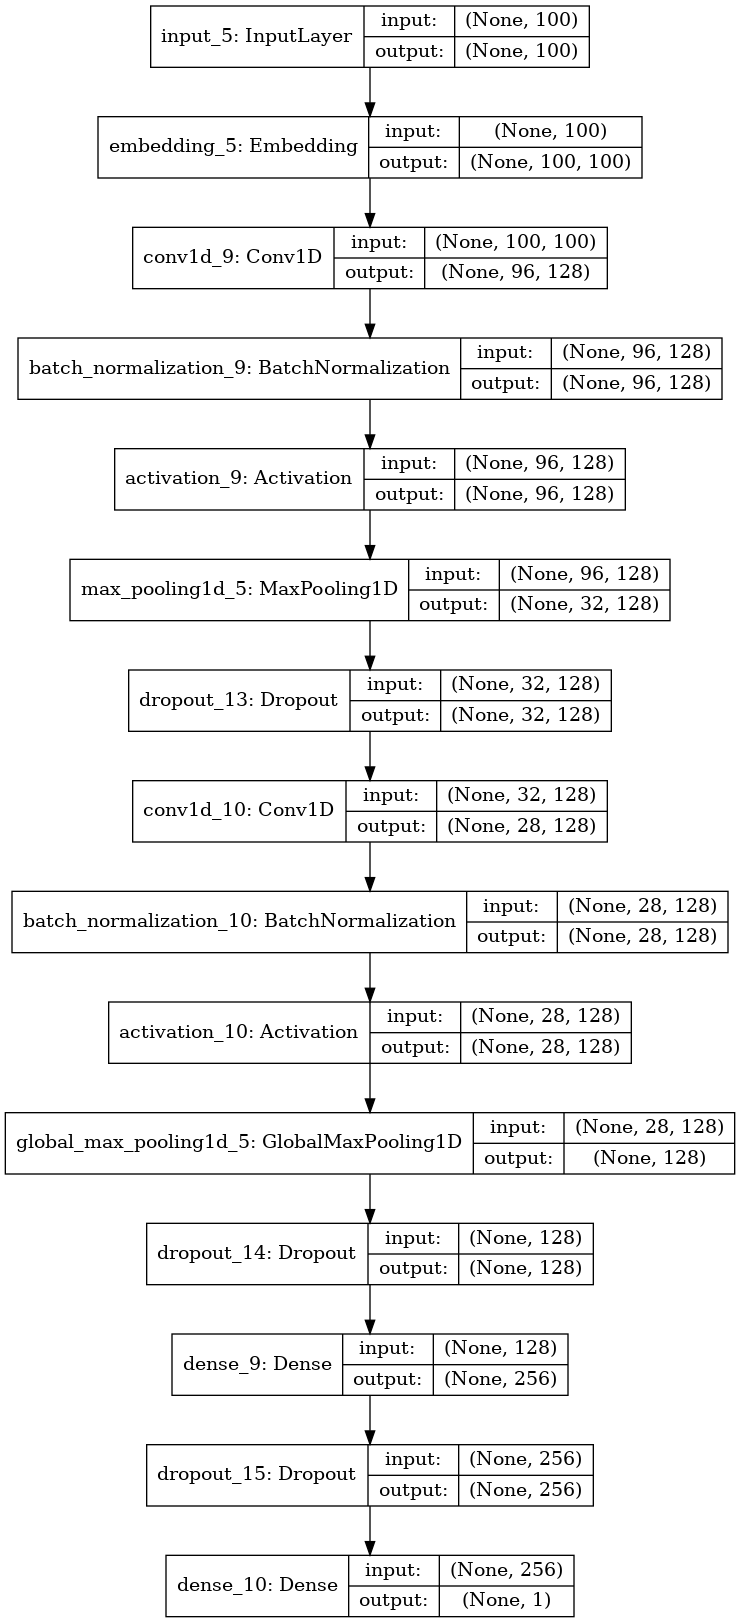
\includegraphics[scale=0.15]{cnn_model.png}
\end{frame}

\begin{frame}
    \frametitle{ELMo Model}
    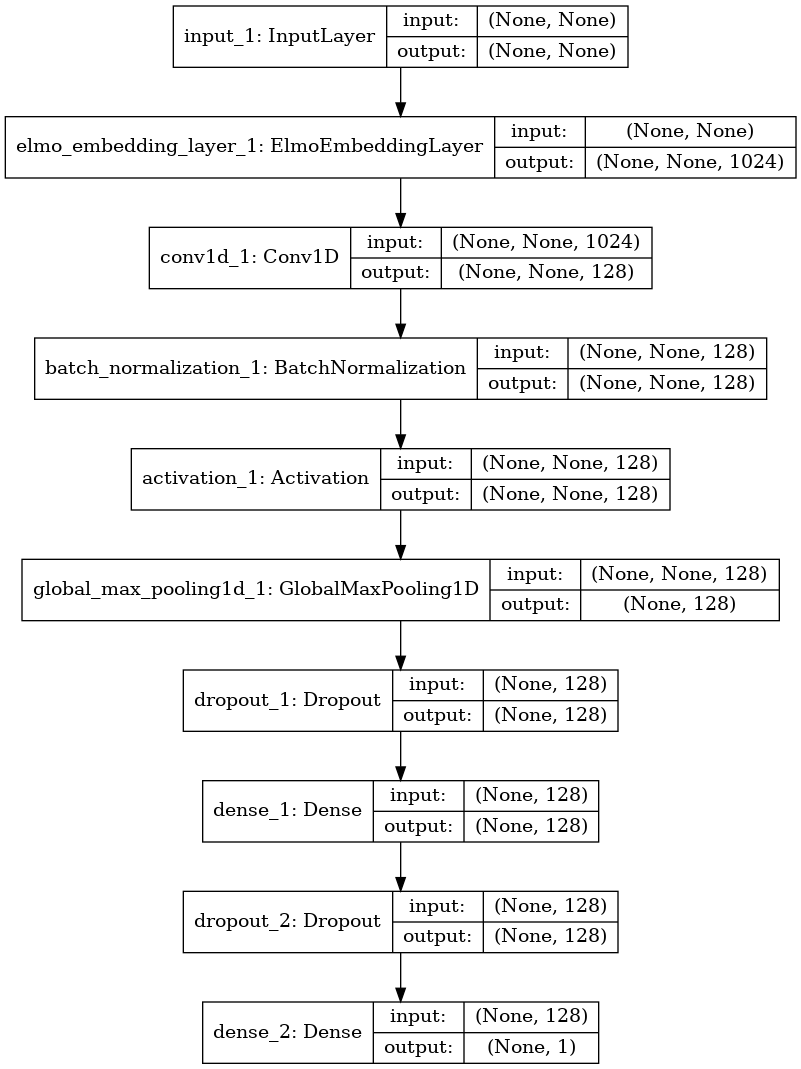
\includegraphics[scale=0.2]{elmo_model.png}
\end{frame}


\section{Conclusion}
\frame{\frametitle{Conclusion}
\begin{itemize}
\item Logistic regression seems to be the best baseline
\item Small improvements possible adding extra features
\item Bypublisher dataset makes it worse
\item It is hard to apply CNN's, not as easy as thought
\item Great resources are needed, also for small machinelearning tasks
\end{itemize}
}

\end{document}

